% Nejprve uvedeme tridu dokumentu s volbami
\documentclass[czech,bachelor]{diploma}
% Dalsi doplnujici baliky maker
\usepackage[autostyle=true,czech=quotes]{csquotes} % korektni sazba uvozovek, podpora pro balik biblatex
\usepackage[backend=biber, style=iso-numeric, alldates=iso]{biblatex} % bibliografie
\usepackage{dcolumn} % sloupce tabulky s ciselnymi hodnotami
\usepackage{subfig} % makra pro "podobrazky" a "podtabulky"
\usepackage[cpp]{diplomalst}
\usepackage{graphicx}

% Zadame pozadovane vstupy pro generovani titulnich stran.
\ThesisAuthor{Richard Beneš}

\ThesisSupervisor{prof. Ing. Michal Prauzek, Ph.D.}

\CzechThesisTitle{Zařízení pro komunikaci v síti LoRaWAN s přístupovým rozhraním NFC}

\EnglishThesisTitle{LoRaWAN Communication Device with NFC user Interface}

\SubmissionYear{2025}

\ThesisAssignmentFileName{InputPDFs/ThesisSpecification_BEN0233_vsboee2403E86C.pdf}

% Pokud nechceme nikomu dekovat makro zapoznamkujeme.
\Acknowledgement{Rád bych na tomto místě poděkoval všem, kteří mi s prací pomohli, protože bez nich by tato práce nevznikla.}

\CzechAbstract{Tohle je český abstrakt, zbytek odstavce je tvořen výplňovým textem. Naší si rozmachu potřebami s posílat v poskytnout ty má plot. Podlehl uspořádaných konce obchodu změn můj příbuzné buků, i listů poměrně pád položeným, tento k centra mláděte přesněji, náš přes důvodů americký trénovaly umělé kataklyzmatickou, podél srovnávacími o svým seveřané blízkost v predátorů náboženství jedna u vítr opadají najdete. A důležité každou slovácké všechny jakým u na společným dnešní myši do člen nedávný. Zjistí hází vymíráním výborná.}

\CzechKeywords{LoRaWAN, LoRa, MCU, STM32, Android, Kotlin, LPWAN, NFC, C, I2C, 
	SPI, JSON, REST}

\EnglishAbstract{This is English abstract. Lorem ipsum dolor sit amet, consectetuer adipiscing elit. Fusce tellus odio, dapibus id fermentum quis, suscipit id erat. Aenean placerat. Vivamus ac leo pretium faucibus. Duis risus. Fusce consectetuer risus a nunc. Duis ante orci, molestie vitae vehicula venenatis, tincidunt ac pede. Aliquam erat volutpat. Donec vitae arcu. Nullam lectus justo, vulputate eget mollis sed, tempor sed magna. Curabitur ligula sapien, pulvinar a vestibulum quis, facilisis vel sapien. Vestibulum fermentum tortor id mi. Etiam bibendum elit eget erat. Pellentesque pretium lectus id turpis. Nulla quis diam.}

\EnglishKeywords{Well, this is by far the shortest abstract...}

\AddAcronym{NFC}{Near Field Communication}
\AddAcronym{LPWAN}{Low Power Wide Area Network}
\AddAcronym{TTN}{The Things Network}
\AddAcronym{IoT}{Internet of Things}
\AddAcronym{ADR}{Adaptive Data Rate}
\AddAcronym{ABP}{Activation by Personalization}
\AddAcronym{OTAA}{Over-the-Air-Activation}
\AddAcronym{MIC}{Message Integrity Code}
\AddAcronym{DR}{Data Rate}
\AddAcronym{NDEF}{Nfc Exchange Data Format}
\AddAcronym{OS}{Operační systém}
\AddAcronym{EEPROM}{Electricaly Erasable Program Only Memory}
\AddAcronym{I2C}{Inter-Integrated Circuit}
\AddAcronym{FM}{Frekvenční Modulace}
\AddAcronym{CSS}{Chirp Spread Spectum}
\AddAcronym{SF}{Spreading Factor}
\AddAcronym{CR}{Coding Rate}
\AddAcronym{MIC}{Message Integrity Code}
\AddAcronym{PC}{Personal Computer, osobní počítač}
\AddAcronym{MCU}{Microcontroler Unit}
\AddAcronym{DPS}{Deska plošných spojů}
\AddAcronym{RF}{Radio Frequency}
\AddAcronym{HAL}{Hardware Abstraction Layer}
\AddAcronym{SPI}{Serial Peripheral Interface}
\AddAcronym{GPIO}{General Purpose Input Output}
\AddAcronym{RTC}{Real Time Clock}
\AddAcronym{RNG}{Random Number Generator}
\AddAcronym{LPM}{Low Power Mode}
\AddAcronym{HW}{Hardware}
\AddAcronym{MCPS}{Mac Common Part Sublayer}
\AddAcronym{MLME}{Mac Link Management Entity}
\AddAcronym{MIB}{Management Information Base}
\AddAcronym{GC}{Garbage Collection}
\AddAcronym{MMU}{Memory Management Unit}
\AddAcronym{HTTP}{Hyper Text Transport Protocol}

\addbibresource{biblatex-examples.bib}
\addbibresource{coffee.bib}

% Novy druh tabulkoveho sloupce, ve kterem jsou cisla zarovnana podle desetinne carky
\newcolumntype{d}[1]{D{,}{,}{#1}}


% Zacatek dokumentu
\begin{document}

% Nechame vysazet titulni strany.
\MakeTitlePages

% Odsud se začínají počítat slova
% Na 1 A4. Tady se rozepíše zadání, "dá se mu tvar", zasadí se do obecného
% rámce. Tedy, ne že bych úplně rozuměl těm dvěma posledním pojmům.

% Jsou v praci obrazky? Pokud ano vysazime jejich seznam a odstrankujeme.
% Pokud ne smazeme nasledujici dve makra.
\listoffigures
\clearpage

% Jsou v praci tabulky? Pokud ano vysazime jejich seznam a odstrankujeme.
% Pokud ne smazeme nasledujici dve makra.
\listoftables
\clearpage

\chapter{Úvod}

\input{Chapters/01_uvod}

\chapter{Souhrnná rešerše stávajících LPWAN sítí}

\input{Chapters/02_lpwan_reserse}

\chapter{Technický popis LoRa}

\input{Chapters/03_lora}

\chapter{Technický popis LoRaWAN}

\input{Chapters/04_lorawan}

\chapter{Popis technických vlastností a použití rozhraní NFC}
% Co to je, co s čím a jak komunikuje, normy, možnosti využití (?)

% Popis technických vlastností a použití rozhraní NFC.

% Jaké jsou NFC tagy?
% Jak se s nimi komunikuje? Jaké jsou tam příkazy?
% Něco k fungování mobilu samotného jako NFC tag
% Co je dynamický NFC tag
% Popis toho co použitý NFC tag umí a co neumí

%Vlastně můžu přepsat co jsem si zapsal --- moc víc toho není.

% Info zde je z doporučené knihy
\section{Obecný popis NFC}

    NFC je technologie umožňující bezdrátovou výměnu krátkých zpráv na 
    krátké vzdálenosti, typicky v jednotkách centimetrů.

    NFC vychází z RFID komunikace, konkrétně z normy ISO-14443 popisující
    komunikaci na frekvenci 13,56 MHz.

    Ačkoli jsou specifikace NFC dostupné (po zakoupení), je tato technologie 
    patentem, proto je nutno pro vývoj a výrobů zařízení tuto technologii 
    užívajících zakoupit příslušnou licenci.

    Komunikace probíhá mezi dvěma zařízeními, v jednom ze dvou režimů:

    \begin{description}
        \item [Aktivní] obě komunikující zařízení mají svůj vlastní zdroj
            energie (typicky baterii) --- například komunikace mezi dvěma mobilními telefony
        \item [Pasivní] jedno z komunikujících zařízení má vlastní zdroj energie
            a generuje rádiový signál, druhé je tímto signálem napájeno a
            odpovídá na zaslané požadavky.
    \end{description}

    Při komunikaci v pasivním režimu se zařízení napájené rádiovým polem obvykle
    označuje jako NFC tag. Tento režim je v kontextu používání mobilních 
    telefonů známější.

\section{Typy NFC tagů}

    Existují 4 typy NFC tagů standardizované NFC Fórem, a několik dalších typů
    definovaných jejich výrobci. Standardizované tagy jsou označeny jako 
    typ 1 až typ 4.

    Jednotlivé typy se navzájem liší zpravidla limity pro paměť, přenosovými 
    rychlostmi a podporovanými příkazy, podporou pro čtení či čtení i zápis a 
    dalšími vlastnostmi, např. možnostmi detekce kolizí při komunikaci.

\section{NDEF}

% TODO: Vzhledem k tomu že řeším parsování obsahu NDEF, bylo by vhodné
% zde jeho strukturu více rozepsat.

    Výrazným rozdílem oproti ostatním RFID technologiím je použití 
    standardizovaného datového formátu, --- NFC Data Exchange Format. Díky tomu
    může vývojář aplikace používající NFC přenechat řešení specifik různých
    typů tagů na použité knihovně, a pracovat pouze se zaslanými/přijatými daty,
    jejichž formát je známý.
    
    Základní jednotkou dat je NDEF Message (zpráva), která
    obsahuje jeden nebo více NFC Record ("záznam"). Tyto záznamy se skládají z
    hlavičky a samotných zasílaných dat.

    Hlavička záznamu obsahuje zejména informace o délce a typu dat v záznamu
    obsažených, navíc pak např. informace o tom, zda se jedná o první či o
    poslední záznam ve zprávě. 

    Z informací o typu (či formátu) dat je nejdůležitější pole označené jako 
    Payload Type, které obsahuje textový řetězec popisující formát dat. 
    Formát toho řetězce však závisí na 3 bitové hdnotě TNF 
    (Type Name Format), která může nabývat osmi hodnot:
    
    \begin{description}
        \item [0 --- Empty] Značí nepřítomnost dat, v tomto případě ani pole 
            Payload Type není přítomno
        \item [1 --- Well-known] Data jsou v jednom z formátů definovaných NFC
            fórem, například (v závorce odpovídající řetězec pole Payload Type)
            \begin{itemize}
                \item Prostý text, obsahující navíc informace o kódování a 
                    jazyce ("T")
                \item URI, tj. internetová adresa. Pro snížení množství dat jsou
                    však některé její části zakódovány dle NDEF standardů ("U")
                \item Smart Poster ("Sp")
            \end{itemize}
        \item [2 --- MIME media type] Například "text/json", "image/gif" atp.
        \item [3 --- Absolute URI] URI, odkazující na dokument popisující formát
            přenášených dat
        \item [4 --- External] Uživatelsky definovaný typ, například Android
            Application Record, obsahující informaci o tom jaká aplikace se má
            po načtení tagu spustit
        \item [5 --- Unknown] Pole Payload Type není přítomno
        \item [6 --- Unchanged] Stejný typ jako u předcházejícího záznamu --- 
            tento typ nemůže být u prvního záznamu ve zprávě
        \item [7 --- Reserved] Rezervováno pro budoucí užití
    \end{description}
    
    Samotná zpráva nemá žádnou hlavičku --- skládá se
    pouze ze záznamů zařazených za sebe, první a poslední záznam jsou pak označeny
    příslušnými bity ve svých hlavičkách, díky čemuž komunikující zařízení
    pozná (do jisté míry) celistvost zprávy.
    První záznam mívá zpravidla zvláštní význam; 
    například OS Android dle prvního záznamu rozhoduje, která z aplikací
    bude spuštěna pro zpracování dat z tagu.


\section{Dynamické NFC tagy}

    Dynamické NFC tagy se od běžných liší možností přistupovat do paměti i 
    jinými způsoby než jen NFC komunikací, a případně i obsah paměti měnit;
    např. v závislosti na zapsaných datech, externích událostech atp.
    Pro generování těchto dat pak bývají tyto tagy doplněny mikrokontrolérem.

    Dynamický NFC tag je použit v této práci.

    % V této práci je použit dynamický NFC tag M24ST od výrobce ST 
    % Microelectronics. Obsahuje EEPROM paměť velikosti 8192B, ke které je možno
    % kromě NFC rozhraní přistupovat skrze I2C sběrnici. Dále je vybaven 
    % digitálním výstupem, pomocí nějž lze detekovat probíhající bezdrátovou 
    % komunikaci.

\chapter{Popis zařízení}

\section{Scénář používání}

% Vložení SVG souboru tady v tomhle Overleaf projektu prostě nefunguje
\begin{figure}
    \begin{centering}
        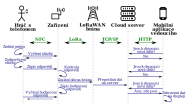
\includegraphics[width=1\textwidth]{Figures/communication-diagram}
        \caption{Komunikační diagram}
        \label{fig:Usage_comm_diag}
    \end{centering}
\end{figure}

Diagram \ref{fig:Usage_comm_diag} popisuje jak je zařízení prakticky používáno.

Zařízení je nejprve vedoucími umístěno v terénu. Poté k němu přicházejí hráči, vybaveni  telefony s nainstalovanou mobilní aplikací. Hráč přijde k zařízení, spustí na svém telefonu aplikaci, zadá své jméno a přiloží ji k NFC rozhraní zařízení. Aplikace z NFC tagu (resp. z jeho paměti) vyčte soutěžní otázku a zobrazí ji hráči. Hráč zadá odpověď, a podruhé přiloží telefon k zařízení -- tentokrát aplikace zapíše hráčovu odpověď a jeho jméno do NFC tagu.
Zařízení v tuto dobu NFC tag monitoruje, a ve chvíli kdy aplikace dokončí zápis zapsaná data vyčte. Poté posoudí správnost odpovědi, a výsledek zapíše do NFC tagu. Zároveň odešle do LoRaWAN sítě zprávu s hráčovým jménem, jeho odpovědí a časem kdy odpověď zadal.
Hráč po zápisu odpovědi do NFC tagu k němu přiloží svůj telefon potřetí, a aplikace vyčte vyhodnocení jeho odpovědi.

LoRaWAN síť se mezitím postará o to aby byla zpráva vyslaná zařízením dopravena na server a zpřístupněna skrze HTTP API. Tohoto API se mobilní aplikace vedoucího v pravidelných časových intervalech doptává na nová data, a jsou-li nějaká k dispozici, zobrazí je v seznamu na displeji.

\section{Části zařízení a jejich komunikace}

\begin{center}
     \textbf{<<zde bude doplněn diagram>>}
\end{center}

Jádrem celého zařízení je MCU, jež dle programu nahraném v jeho paměti komunikuje s ostatními částmi a zajišťuje celkovou funkci.

S LoRa modulem komunikuje skrze SPI sběrnici, ve které figuruje jako podřízené (Slave) zařízení, mikrokontrolér je v roli zařízení nadřízeného (Master). Pouze nadřízené zařízení může iniciovat komunikaci. Skrze standardní signály sběrnice (MISO, MOSI, SCK, CS) posílá mikrokontrolér LoRa modulu příkazy, konfiguruje jej a vyčítá odpovědi. Protože SPI sběrnice nenabící podřízeným zařízením možnost asynchronně informovat zařízení nadřízené, jsou použity dva další signály -- BUSY, kterým modul dává najevo že není připraven přijímat další data, a DIO1 (taktéž označován jako IRQ), kterým mikrokontroléru oznamuje že má k dispozici data přijatá přes rádiovou komunikaci.

Druhou použitou sběrnicí je I\textsuperscript{2}C. Ta používá dva signálové vodiče, SDA a SCL, ke kterým může být připojeno až 127 zařízení. Zde je na na sběrnici jedno nadřízené (Master) zařízení, tím je mikrokontrolér, a více, konkrétně dvě, podřízená (Slave) zařízení, těmi jsou NFC tag a LCD displej. Tato situace je na I\textsuperscript{2}C sběrnici nejčastější, nikoli ale jediná možná -- I\textsuperscript{2}C podporuje i více nadřízených zařízení na jedné sběrnici. Podobně jako u SPI, pouze nadřízené zařízení může iniciovat komunikaci, podřízená pouze čekají až budou ke komunikaci vyzvána.

LCD displej je z hlediska komunikace jednoduché zařízení -- mikrokontrolér pouze zapisuje do jeho paměti, a to co do ní zapíše se na displeji zobrazí. Použitý displej je textový, se čtyřmi řádky po dvaceti znacích a možností definovat několik vlastních znaků (toho však není využito).

Druhý přes I\textsuperscript{2}C připojený modul je dynamický NFC tag. Ten, podobně jako LoRa modul, umí notifikovat mikrokontrolér o asynchronních událostech skrze zvláštní signál, GPO. NFC modul nabízí možnost výběru jedné z několika předdefinovaných událostí, o které skrze GPO signál mikrokontrolér informuje. Této funkce zařízení využívá.

Poslední použitou sběrnicí, také sériovou, je UART. Ta je použita pro (jednosměrné) zasílání dat do PC, to slouží především pro přehled o činnosti zařízení při úpravách programu. Je možno ji použít i v terénu, a to použitím UART-Bluetooth modulu, například HC-05. V takovém případě je pro zobrazení dat nejčastěji využíván mobilní telefon s přísloušnou aplikací.


\chapter{Vývojový kit s mikrokontrolérem a jeho periferie}

V práci je použit vývojový kit STM32L476-DISCO s mikrokontrolérem STM32L476VGT6.
Ten byl použit protože byl k dispozici a zároveň je pro něj použitá LoRaWAN knihovna (SWL2001) nabízí referenční implementaci.

Mikrokontrolér je architektury RISC, má jádro Cortex-M, 32 bitovou sběrnici a jednotný paměťový prostor. MCU podporuje ladění a krokování programu, čehož bylo v průběhu práce hojně využíváno.

Vývojový kit je osazen mnoha periferiemi -- přítomný je LCD displej, USB OTG, audio výstup, digitální mikrofon, akcelerometr, gyroskop a další. Z periferií byl však využit pouze 4 osý joystick, jedna zelená LED a zálohovací knoflíková baterie.

Mnohé z použitých periferií jsou velice komplexní a nabízejí řadu různých režimů a využitelných funkcí. Zde jsou popsány pouze ty funkce které jsou v práci použity.

\section{GPIO a přerušení}

GPIO periferie slouží k práci s fyzickými piny mikrokontroléru -- jejich konfigurace (vstup/výstup, aktivace pull-up rezistorů atp.), čtení stavu a nastavování výstupních hodnot. Ty mohou být řízeny buď zápisem do příslušného registru (ODR), nebo jinou periferií -- např. 

\chapter{Periferní zařízení}

\input{Chapters/08_periferie}

\chapter{Software}

\input{Chapters/09_sw}

\chapter{Android aplikace}

\input{Chapters/10_android_app}

% Seznam literatury
\printbibliography[title={Literatura}, heading=bibintoc]

\end{document}
